\chapter{RESULTS AND DISCUSSION}
This chapter describes the implementation and results of the empirical analysis
outlined above.  Each section of this chapter details one of the three main
tasks of the empirical analysis.  The first task is to create synthetic data,
the second to train the SOMs and finally to apply the diagnostics.

\section{Data}
%The data will be generated with the common technique of rejection sampling,
%where n high dimensional seeds are chosen at random, samples will be taken
%at random from a uniform distribution, if the sample falls with in radius r of
%any seed it is accepted, if it does not, single random number is drawn, if that
%number is \(<\) 0.05\% the sample is accepted as noise, else the sample is rejected.
The training data will be generated using a Gaussian cluster generator as
described by \cite{handl}.  To generate the data we have to decide how many
clusters to create and how many dimensions to use.  In order to set these
parameters appropriately we will first explore how the internal variance
responds to adjustments in their value.

To accomplish this twenty test datasets are generated and used to train each
topology, for a total of eighty SOMs. As shown in table \ref{ivtable1} all topologies
seem to respond similarly. The internal variance of the SOM increases as we
add dimensions and decreases as we add clusters. Based on these results, it was
decided that five dimensions and ten clusters was a reasonable choice. Five
dimensions is easier to work with than larger numbers and should yield more
information than two dimensions.

The results shown in \ref{ivtable1} are in line with what one would expect.
The SOM has a hard time organizing the random datasets (the datasets with no
clusters) resulting more competition between neurons and high internal
variances.

\begin{table}
\caption{Mean Internal Variance}
\label{ivtable1}
\centering

\subtable[Rook Topology]{
  \begin{tabular}{|c||c|c|c|c|}
  \hline
  &\multicolumn{4}{c|}{\textbf{Dimensions}}\\
  \textbf{Clusters} & \multicolumn{1}{c}{\textbf{2}} &
  \multicolumn{1}{c}{\textbf{5}} & \multicolumn{1}{c}{\textbf{10}} &
  \multicolumn{1}{c|}{\textbf{20}}\\
  \hline
  \hline
  \textbf{0} & 0.0206& 0.2796& 0.7300& 1.4173 \\
  \hline
  \textbf{2} & 0.0114& 0.1140& 0.2598& 0.4930 \\
  \hline
  \textbf{5} & 0.0116& 0.0989& 0.2213& 0.4623 \\
  \hline
  \textbf{10} & 0.0117& 0.0920& 0.2071& 0.4207 \\
  \hline
  \textbf{20} & 0.0120& 0.0851& 0.2020& 0.4059 \\
  \hline
  \end{tabular}
  \label{ivtable:rook}
}
\subtable[Hexagonal Topology]{
  \begin{tabular}{|c||c|c|c|c|}
  \hline
  &\multicolumn{4}{c|}{\textbf{Dimmensions}}\\
  \textbf{Clusters} & \multicolumn{1}{c}{\textbf{2}} &
  \multicolumn{1}{c}{\textbf{5}} & \multicolumn{1}{c}{\textbf{10}} &
  \multicolumn{1}{c|}{\textbf{20}}\\
  \hline
  \hline
  \textbf{0} & 0.0205& 0.2784& 0.7336& 1.4192 \\
  \hline
  \textbf{2} & 0.0109& 0.1134& 0.2585& 0.4930 \\
  \hline
  \textbf{5} & 0.0111& 0.0997& 0.2229& 0.4598 \\
  \hline
  \textbf{10} & 0.0114& 0.0922& 0.2085& 0.4236 \\
  \hline
  \textbf{20} & 0.0117& 0.0860& 0.2008& 0.4041 \\
  \hline
  \end{tabular}
  \label{ivtable1:hex}
}
\subtable[Spherical Topology]{
  \begin{tabular}{|c||c|c|c|c|}
  \hline
  &\multicolumn{4}{c|}{\textbf{Dimensions}}\\
  \textbf{Clusters} & \multicolumn{1}{c}{\textbf{2}} &
  \multicolumn{1}{c}{\textbf{5}} & \multicolumn{1}{c}{\textbf{10}} &
  \multicolumn{1}{c|}{\textbf{20}}\\
  \hline
  \hline
  \textbf{0} & 0.0207& 0.2661& 0.7131& 1.3997 \\
  \hline
  \textbf{2} & 0.0106& 0.1106& 0.2550& 0.4872 \\
  \hline
  \textbf{5} & 0.0117& 0.0968& 0.2194& 0.4557 \\
  \hline
  \textbf{10} & 0.0118& 0.0910& 0.2051& 0.4174 \\

  \hline
  \textbf{20} & 0.0123& 0.0844& 0.1989& 0.4017 \\
  \hline
  \end{tabular} 
  \label{ivtable1:graph}
} 
\subtable[Geodesic Sphere Topology]{
  \begin{tabular}{|c||c|c|c|c|}
  \hline
  &\multicolumn{4}{c|}{\textbf{Dimmensions}}\\
  \textbf{Clusters} & \multicolumn{1}{c}{\textbf{2}} &
  \multicolumn{1}{c}{\textbf{5}} & \multicolumn{1}{c}{\textbf{10}} &
  \multicolumn{1}{c|}{\textbf{20}}\\
  \hline
  \hline
  \textbf{0} & 0.0207& 0.2657& 0.7140& 1.3981 \\
  \hline
  \textbf{2} & 0.0111& 0.1110& 0.2553& 0.4870 \\
  \hline
  \textbf{5} & 0.0112& 0.0966& 0.2204& 0.4546 \\
  \hline
  \textbf{10} & 0.0117& 0.0908& 0.2058& 0.4183 \\
  \hline
  \textbf{20} & 0.0120& 0.0857& 0.1995& 0.3994 \\
  \hline
  \end{tabular}
  \label{ivtable1:geodesic}
}
\end{table}






\section{Internal variance vs. first-order neighborhood size}
As outlined in section \ref{q1} we can look at how the internal variance
changes with with respect the degree of a neuron.  

In order to compare the IV accross groups it it necessary to train multiple
soms 
To setup this experiment we
first generate ten synthetic data sets using the method desribed above.  These
data sets will be used to train ten SOMs for each topology.  The reason we
train multiple SOMs for each to is to ensure that we have large enough groups to 
As mentioned in section \ref{q1} the neurons.
With these parameters chosen ten data sets are generated and used to train
SOMs for each topology.  After running ten simulations for the spherical,
hexagonal and rook topologies we find that the mean internal variance seems to
remain fairly stable, this suggests that we can combine the results of each
simulation to compare across topologies. As shown in table \ref{ivtable3}.

\begin{table}
\centering
\caption{Mean IV for each simulation, by topology}
\label{ivtable3}
\begin{tabular}{|c||c|c|c|c|}
\hline
\textbf{Simulation Number} & Geodesic & Graph & Hex & Rook \\
\hline
\hline
\textbf{1} & 0.0966 & 0.0968 & 0.0997 & 0.0989 \\
\hline
\textbf{2} & 0.0875 & 0.0874 & 0.0887 & 0.0886 \\
\hline
\textbf{3} & 0.0807 & 0.0809 & 0.0813 & 0.0814 \\
\hline
\textbf{4} & 0.0816 & 0.0812 & 0.0834 & 0.0823 \\
\hline
\textbf{5} & 0.0912 & 0.0907 & 0.0927 & 0.0929 \\
\hline
\textbf{6} & 0.0943 & 0.0938 & 0.0966 & 0.0944 \\
\hline
\textbf{7} & 0.0905 & 0.0908 & 0.0916 & 0.0929 \\
\hline
\textbf{8} & 0.0789 & 0.0792 & 0.0798 & 0.0797 \\
\hline
\textbf{9} & 0.0984 & 0.0974 & 0.0994 & 0.1001 \\
\hline
\textbf{10} & 0.0900 & 0.0897 & 0.0917 & 0.0910 \\
\hline
\end{tabular} \end{table}



%Currently implemented are the rectangular and spherical topologies, the hexagon
%and geodesic are to be implemented only as graphs.  I.E. the topologies will be
%generated externally and turned into a networkX graph, for use in the graph
%based SOM. The spherical topology also relies on external programs to generate
%the graph structure (spherical voronoi).
\subsection{Restate the Questions}
\textbf{Objective}, Compare the internal variance of observations captured by a given
neuron to that neuron's first-order neighborhood size.

\textbf{Question}, Does the internal variance of a neuron decrease as its first-order
neighborhood size, or degree, increases?



this table shows the means and variances for the degree groups,
\ref{meanvar1}. \footnote{The Combined sizes may not add up to expeded amount.
This is because we can only calculate an IV for neurons which are the BMU of
two or more observations.}

\begin{table}
\caption{Mean IV grouped by a neurons degree for each topology}
\label{meanvar1}
\begin{tabular}{|c||c|c|c||c|c|c||c|c|c||c|c|c|}
\hline
\textbf{Degree Size} & \multicolumn{3}{c||}{\textbf{Geodesic}} &
\multicolumn{3}{c||}{\textbf{Graph}} & \multicolumn{3}{c||}{\textbf{Hex}} &
\multicolumn{3}{c||}{\textbf{Rook}} \\
\hline
& N & MeanIV & VarIV & N & MeanIV & VarIV & N & MeanIV & VarIV & N & MeanIV &
VarIV \\
\hline
2&&&&&&& 20& 0.1109& 0.0010& 40& 0.1123& 0.0007\\ 
3&&&&&&& 223& 0.1054& 0.0010& 918& 0.0997& 0.0009\\ 
4&&&&&&& 507& 0.0980& 0.0009& 5138& 0.0875& 0.0009\\ 
5& 115& 0.0898& 0.0009& 557& 0.0886& 0.0009& 208& 0.0921& 0.0008&&&\\ 
6& 5929& 0.0884& 0.0009& 5034& 0.0883& 0.0009& 5184& 0.0881& 0.0009&&&\\ 
7&&&& 437& 0.0873& 0.0009&&&&&&\\ 
\hline 
Combined& 6044& 0.0884& 0.0009& 6028& 0.0882& 0.0009& 6142& 0.0897& 0.0010&
6096& 0.0895& 0.0009\\ 
\hline
\end{tabular} \end{table}




here are the box plots for the IV. \ref{fRookIV} \ref{fGraphIV} \ref{fHexIV}
\ref{fGeodesicIV}


\begin{figure}
\centering
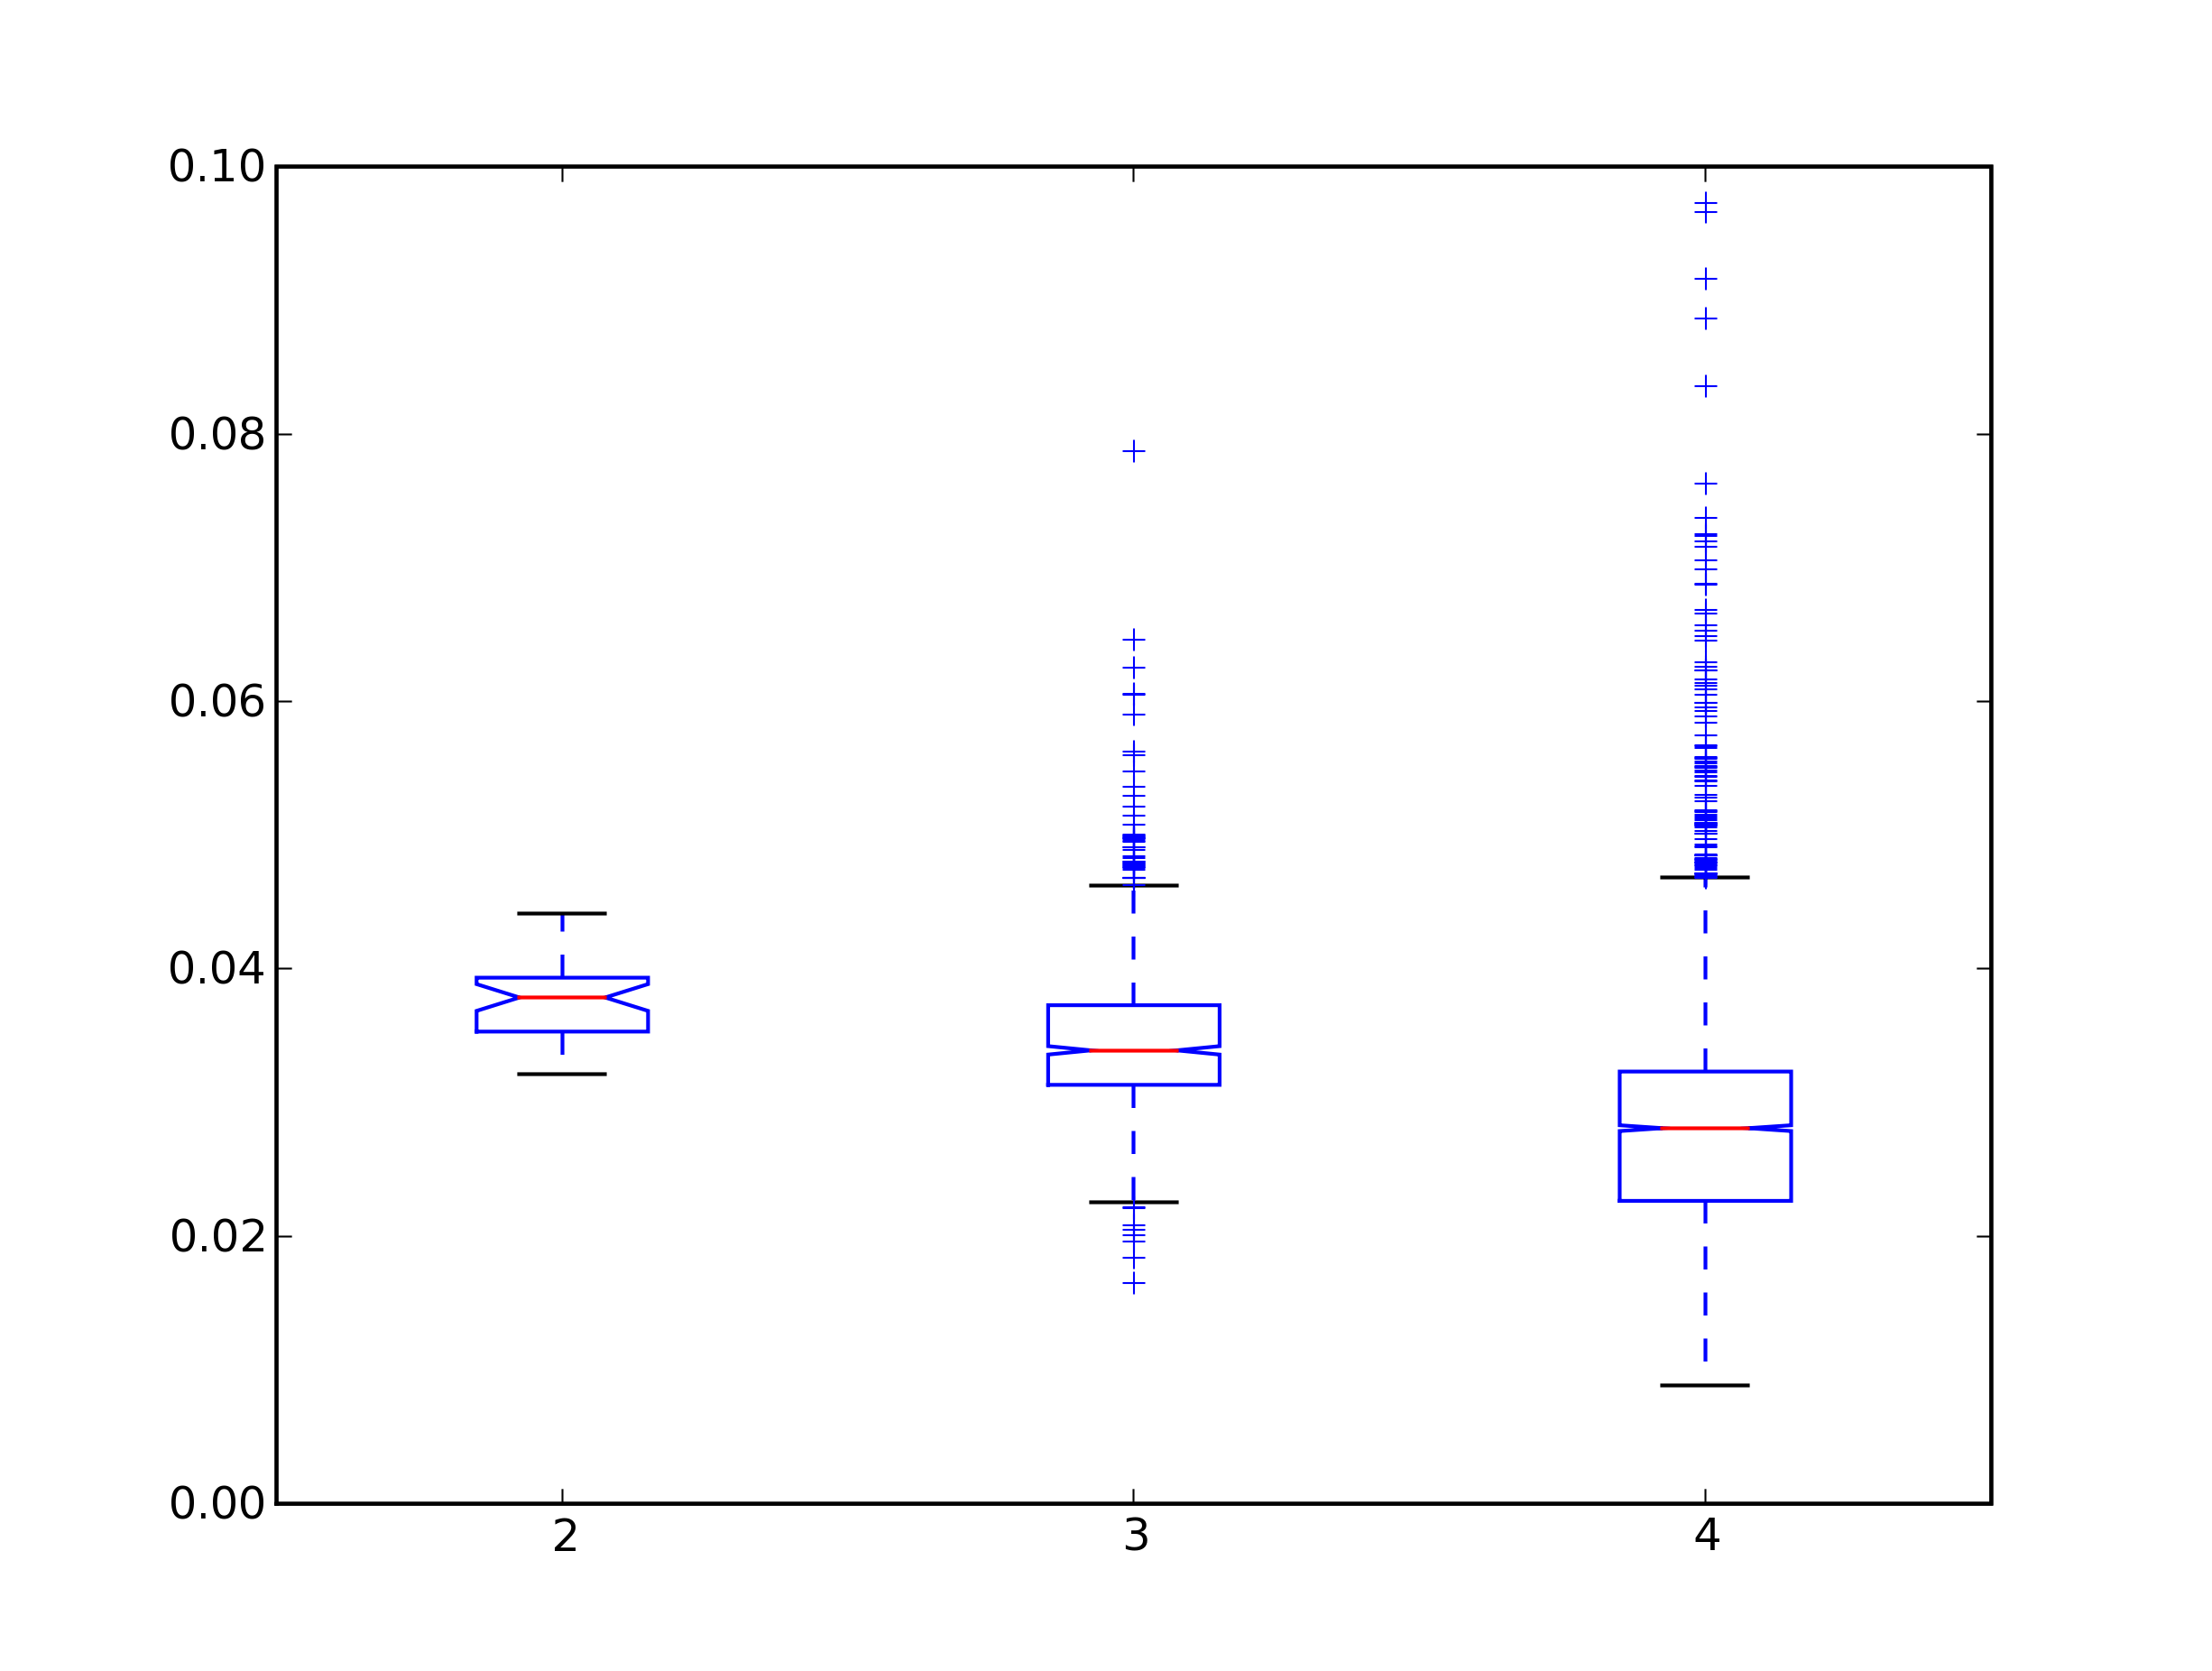
\includegraphics[width=\linewidth]{rook_iv_box.png}
\caption{This shows 4 box plots, each representing one group of neurons in a set
of SOMs trained with the same paremeters.}
\label{fRookIV}
\end{figure}

\begin{figure}
\centering
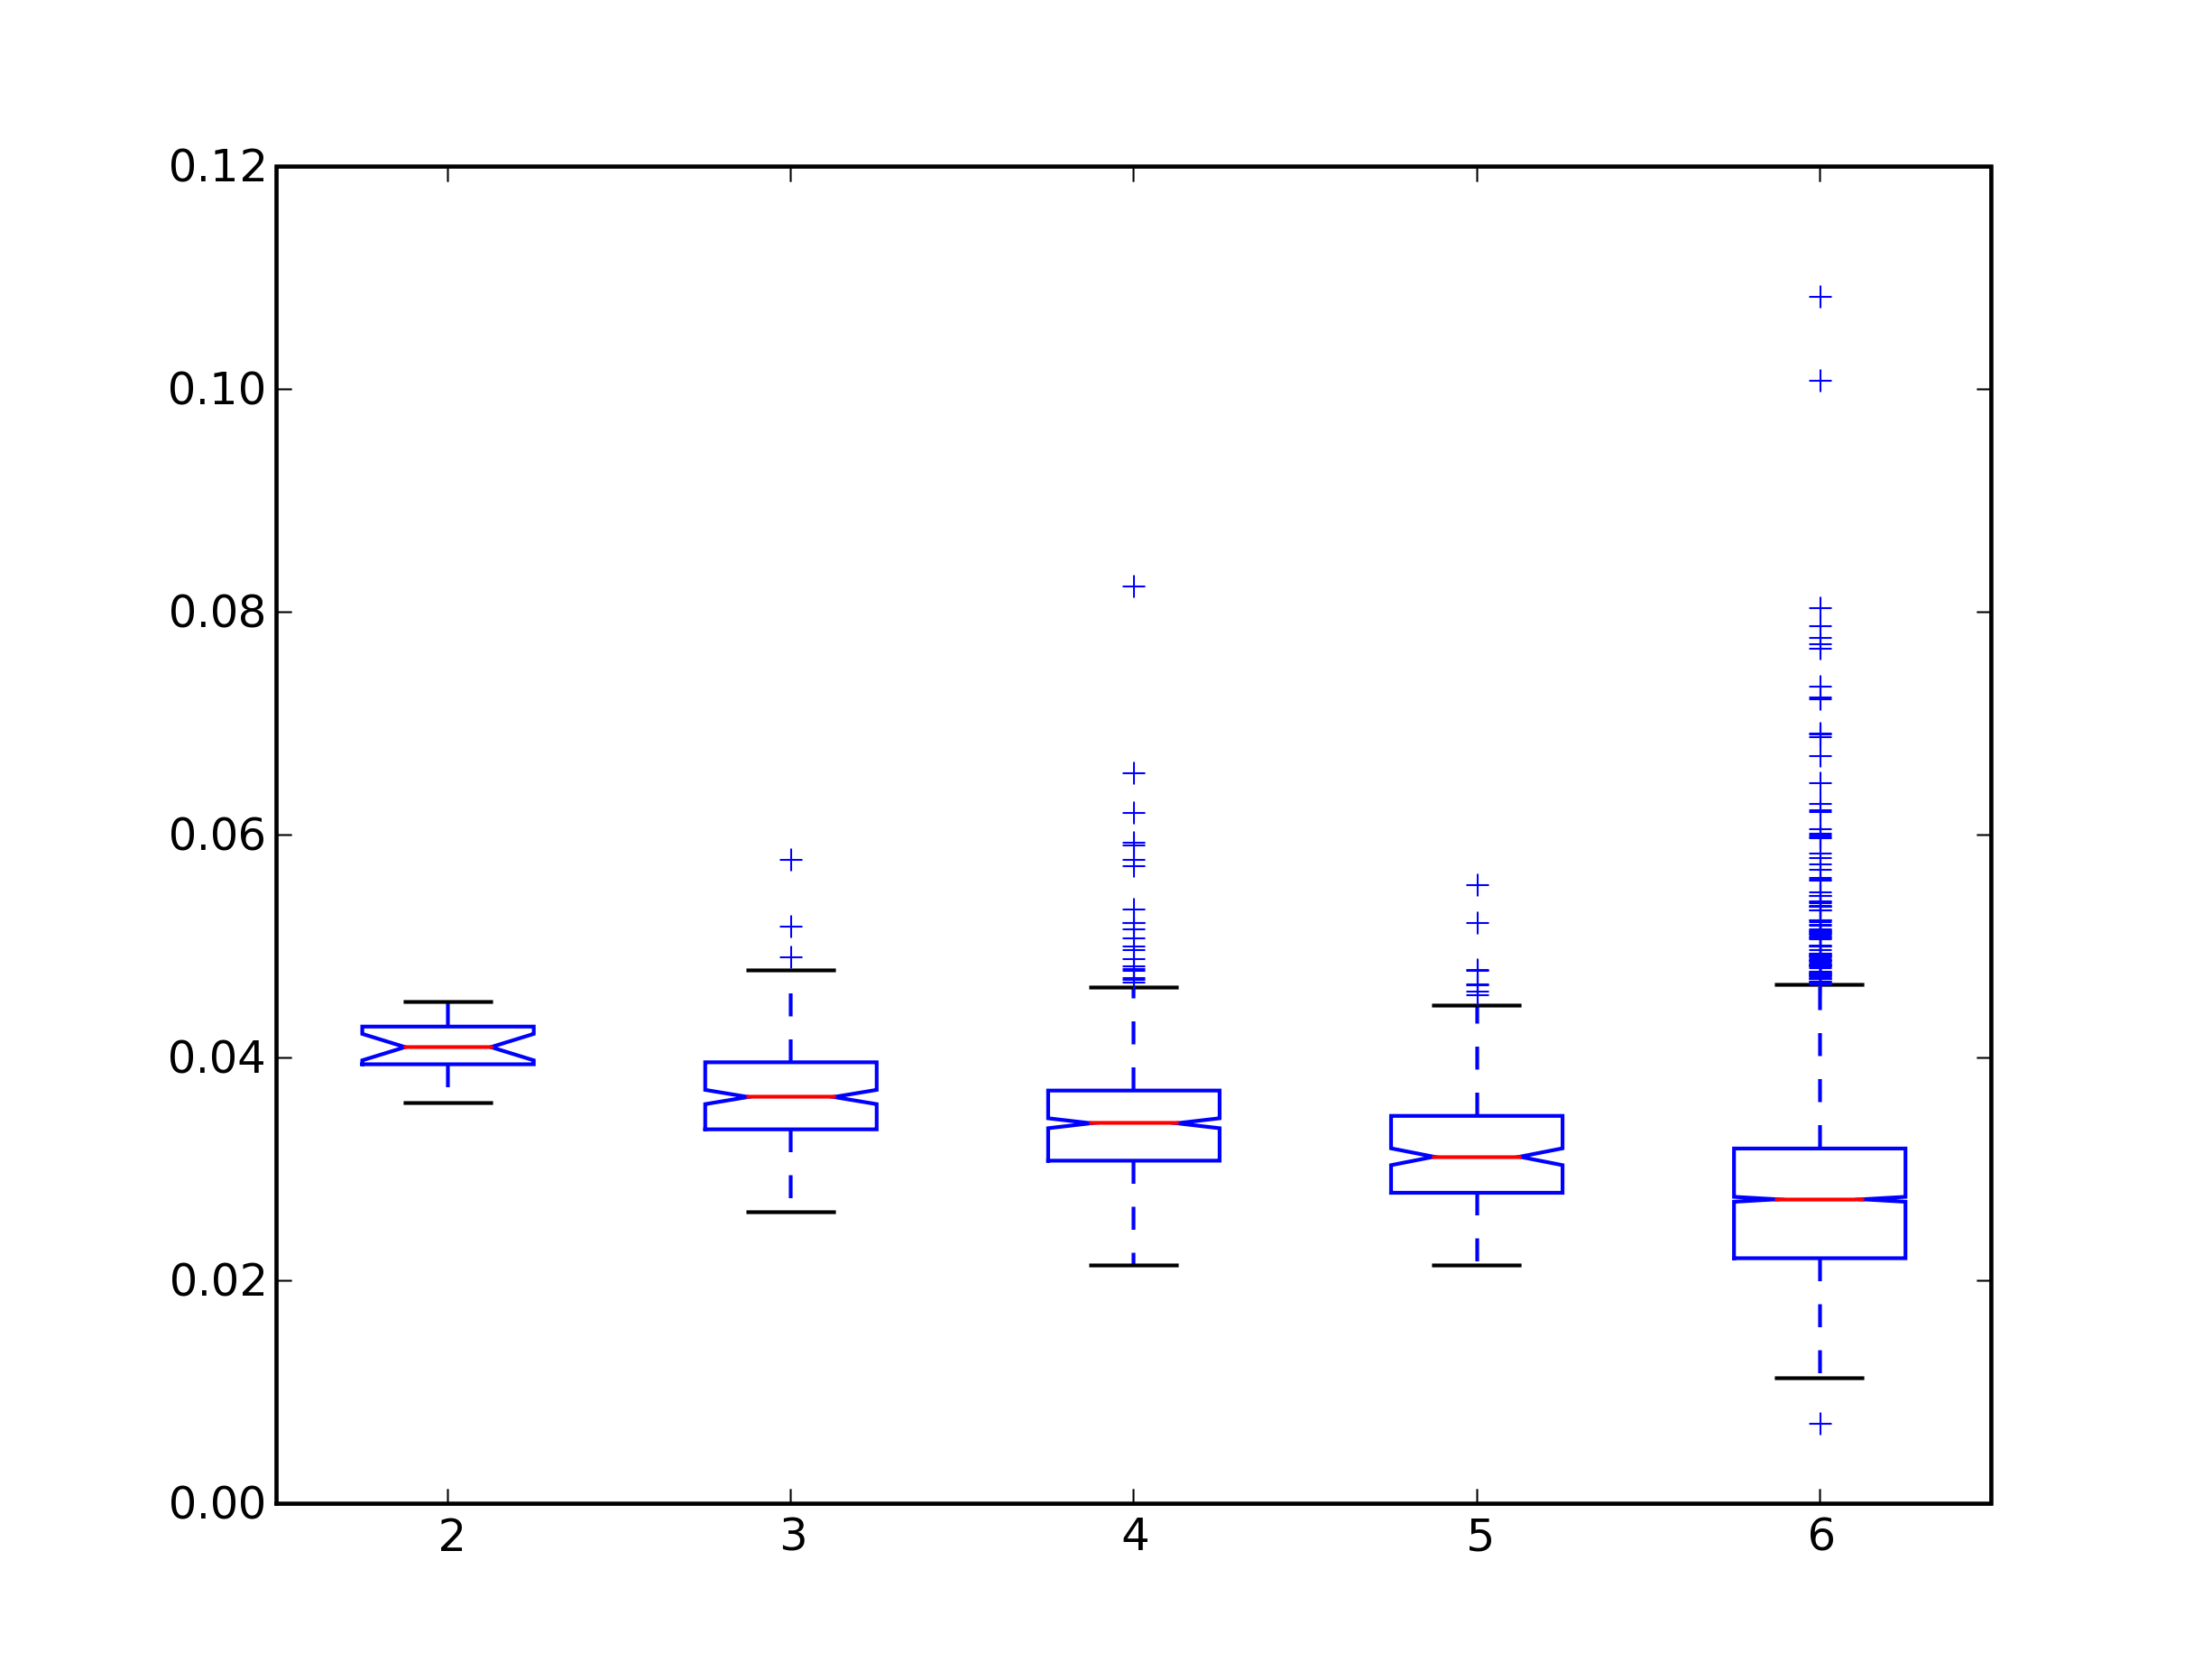
\includegraphics[width=\linewidth]{hex_iv_box.png}
\caption{This shows 4 box plots, each representing one group of neurons in a set
of SOMs trained with the same paremeters.}
\label{fHexIV}
\end{figure}

\begin{figure}
\centering
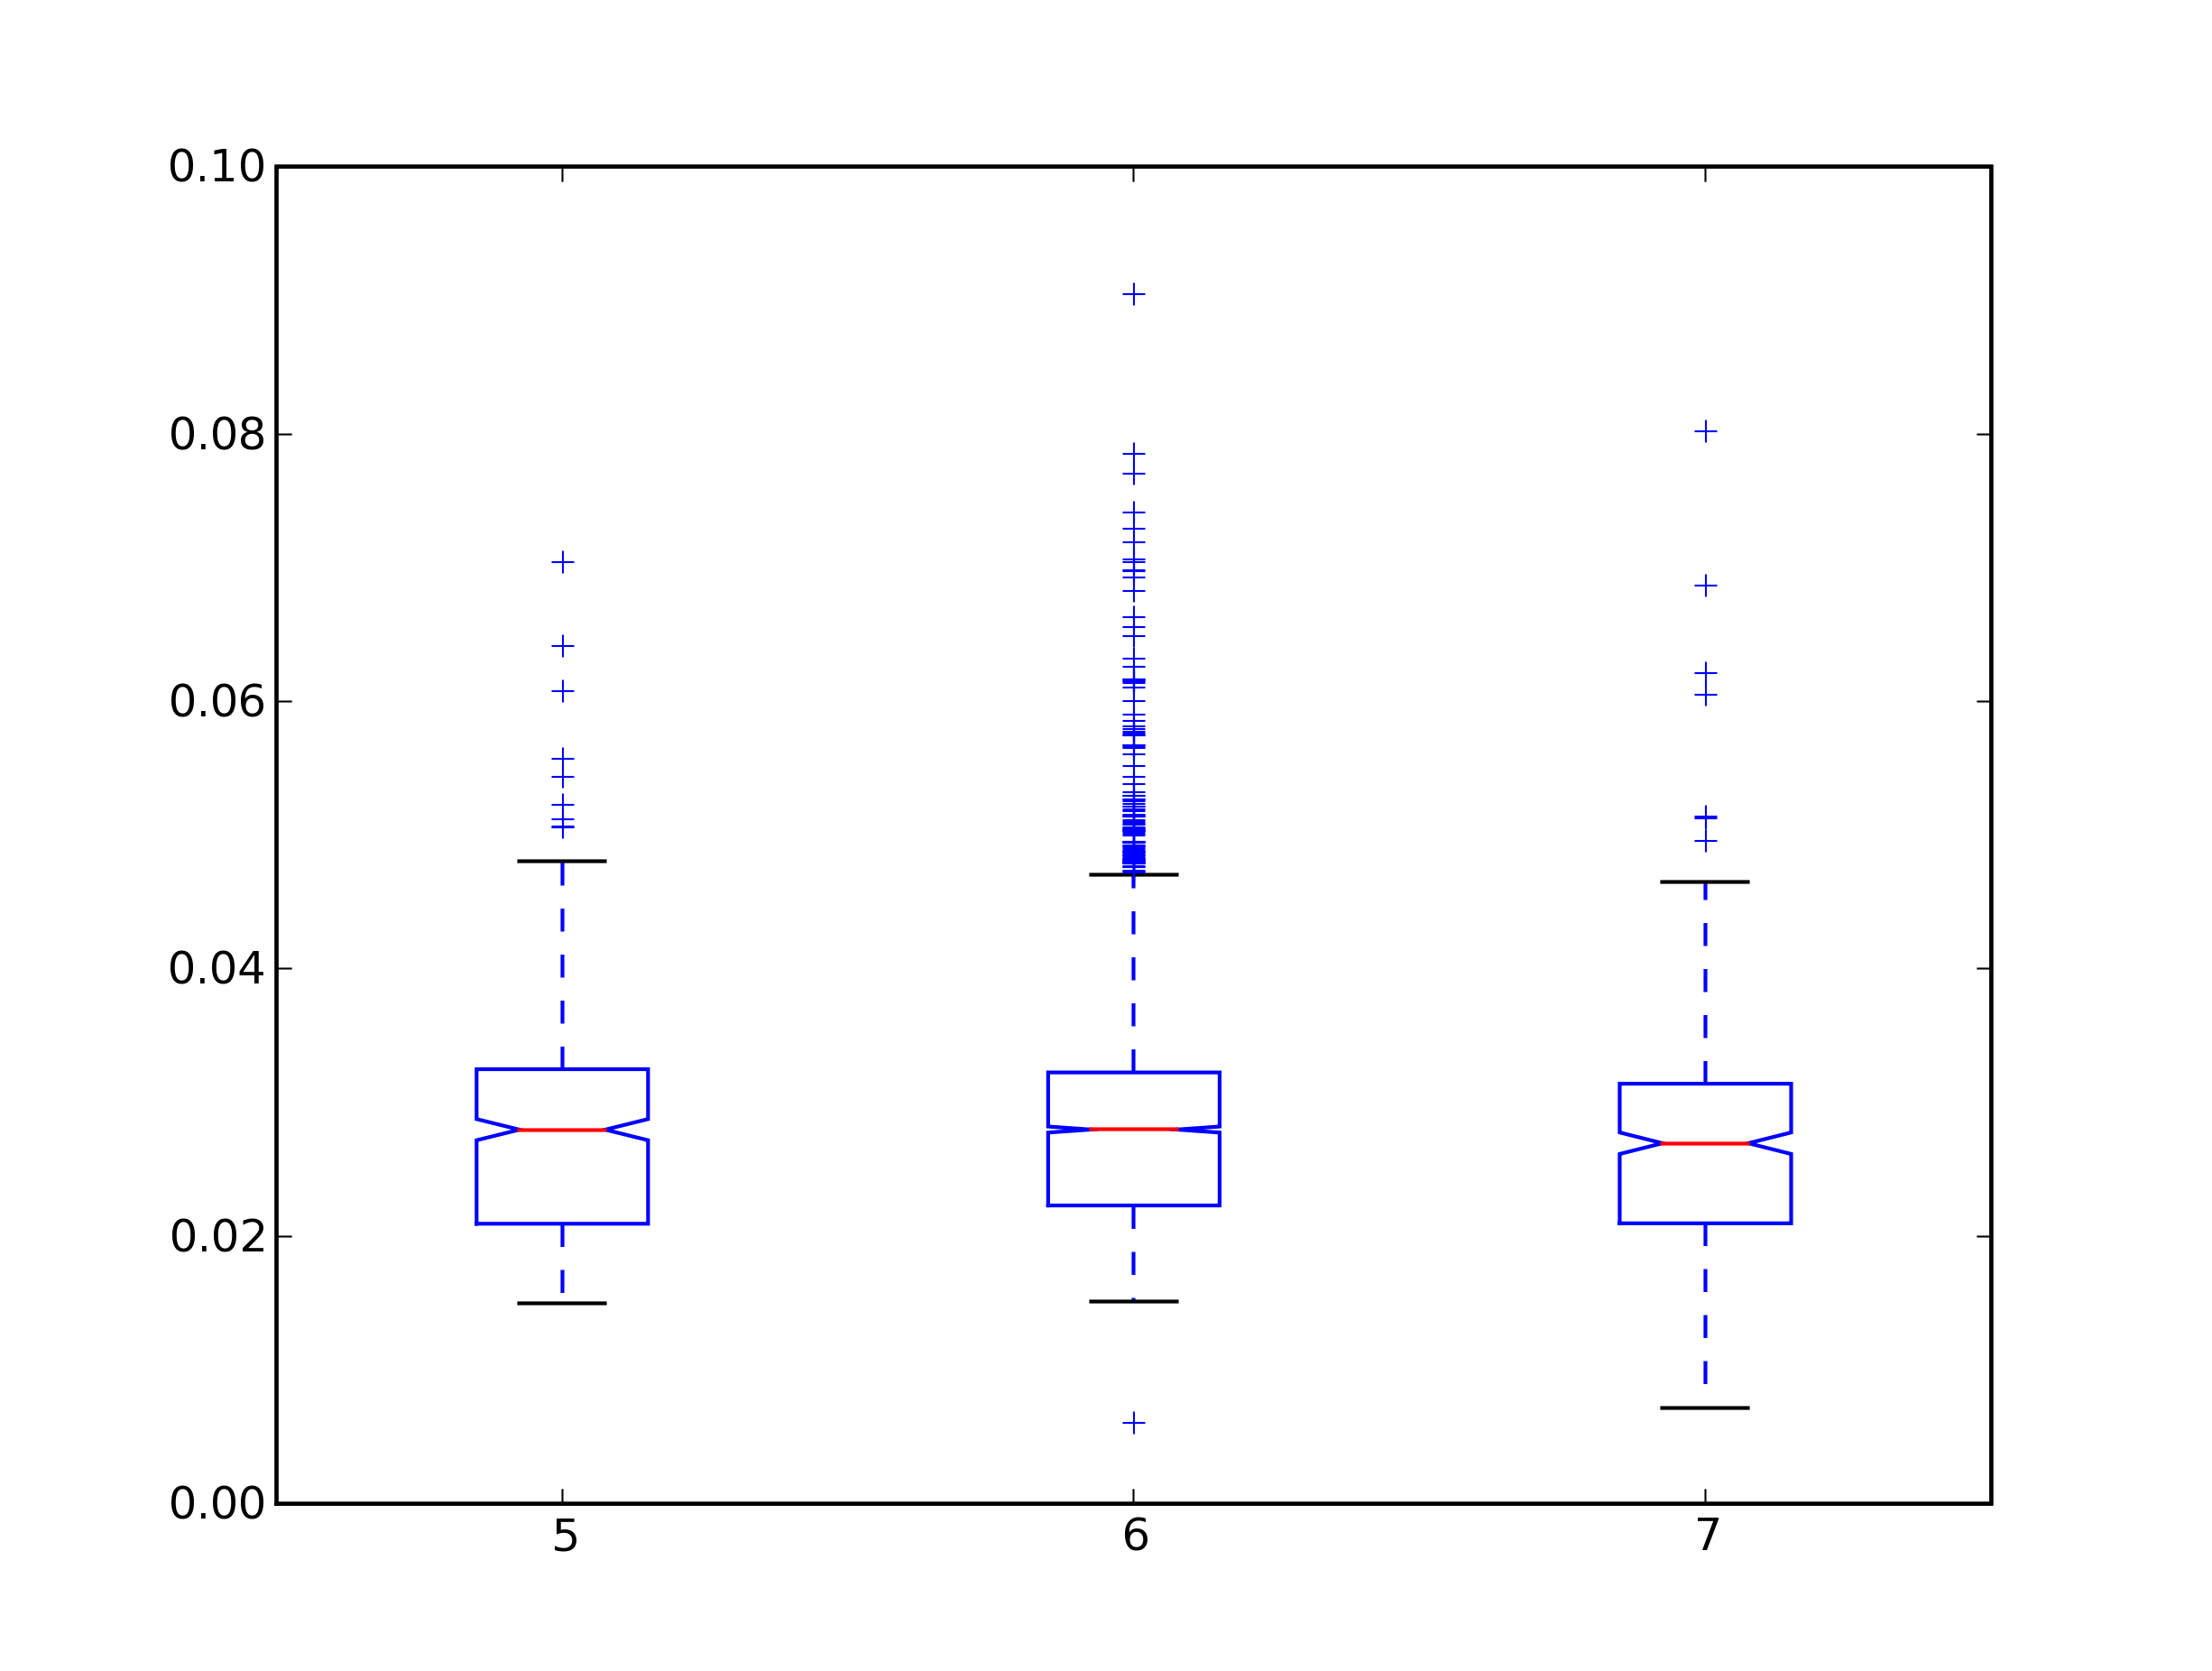
\includegraphics[width=\linewidth]{graph_iv_box.png}
\caption{This shows 4 box plots, each representing one group of neurons in a set
of SOMs trained with the same paremeters.}
\label{fGraphIV}
\end{figure}

\begin{figure}
\centering
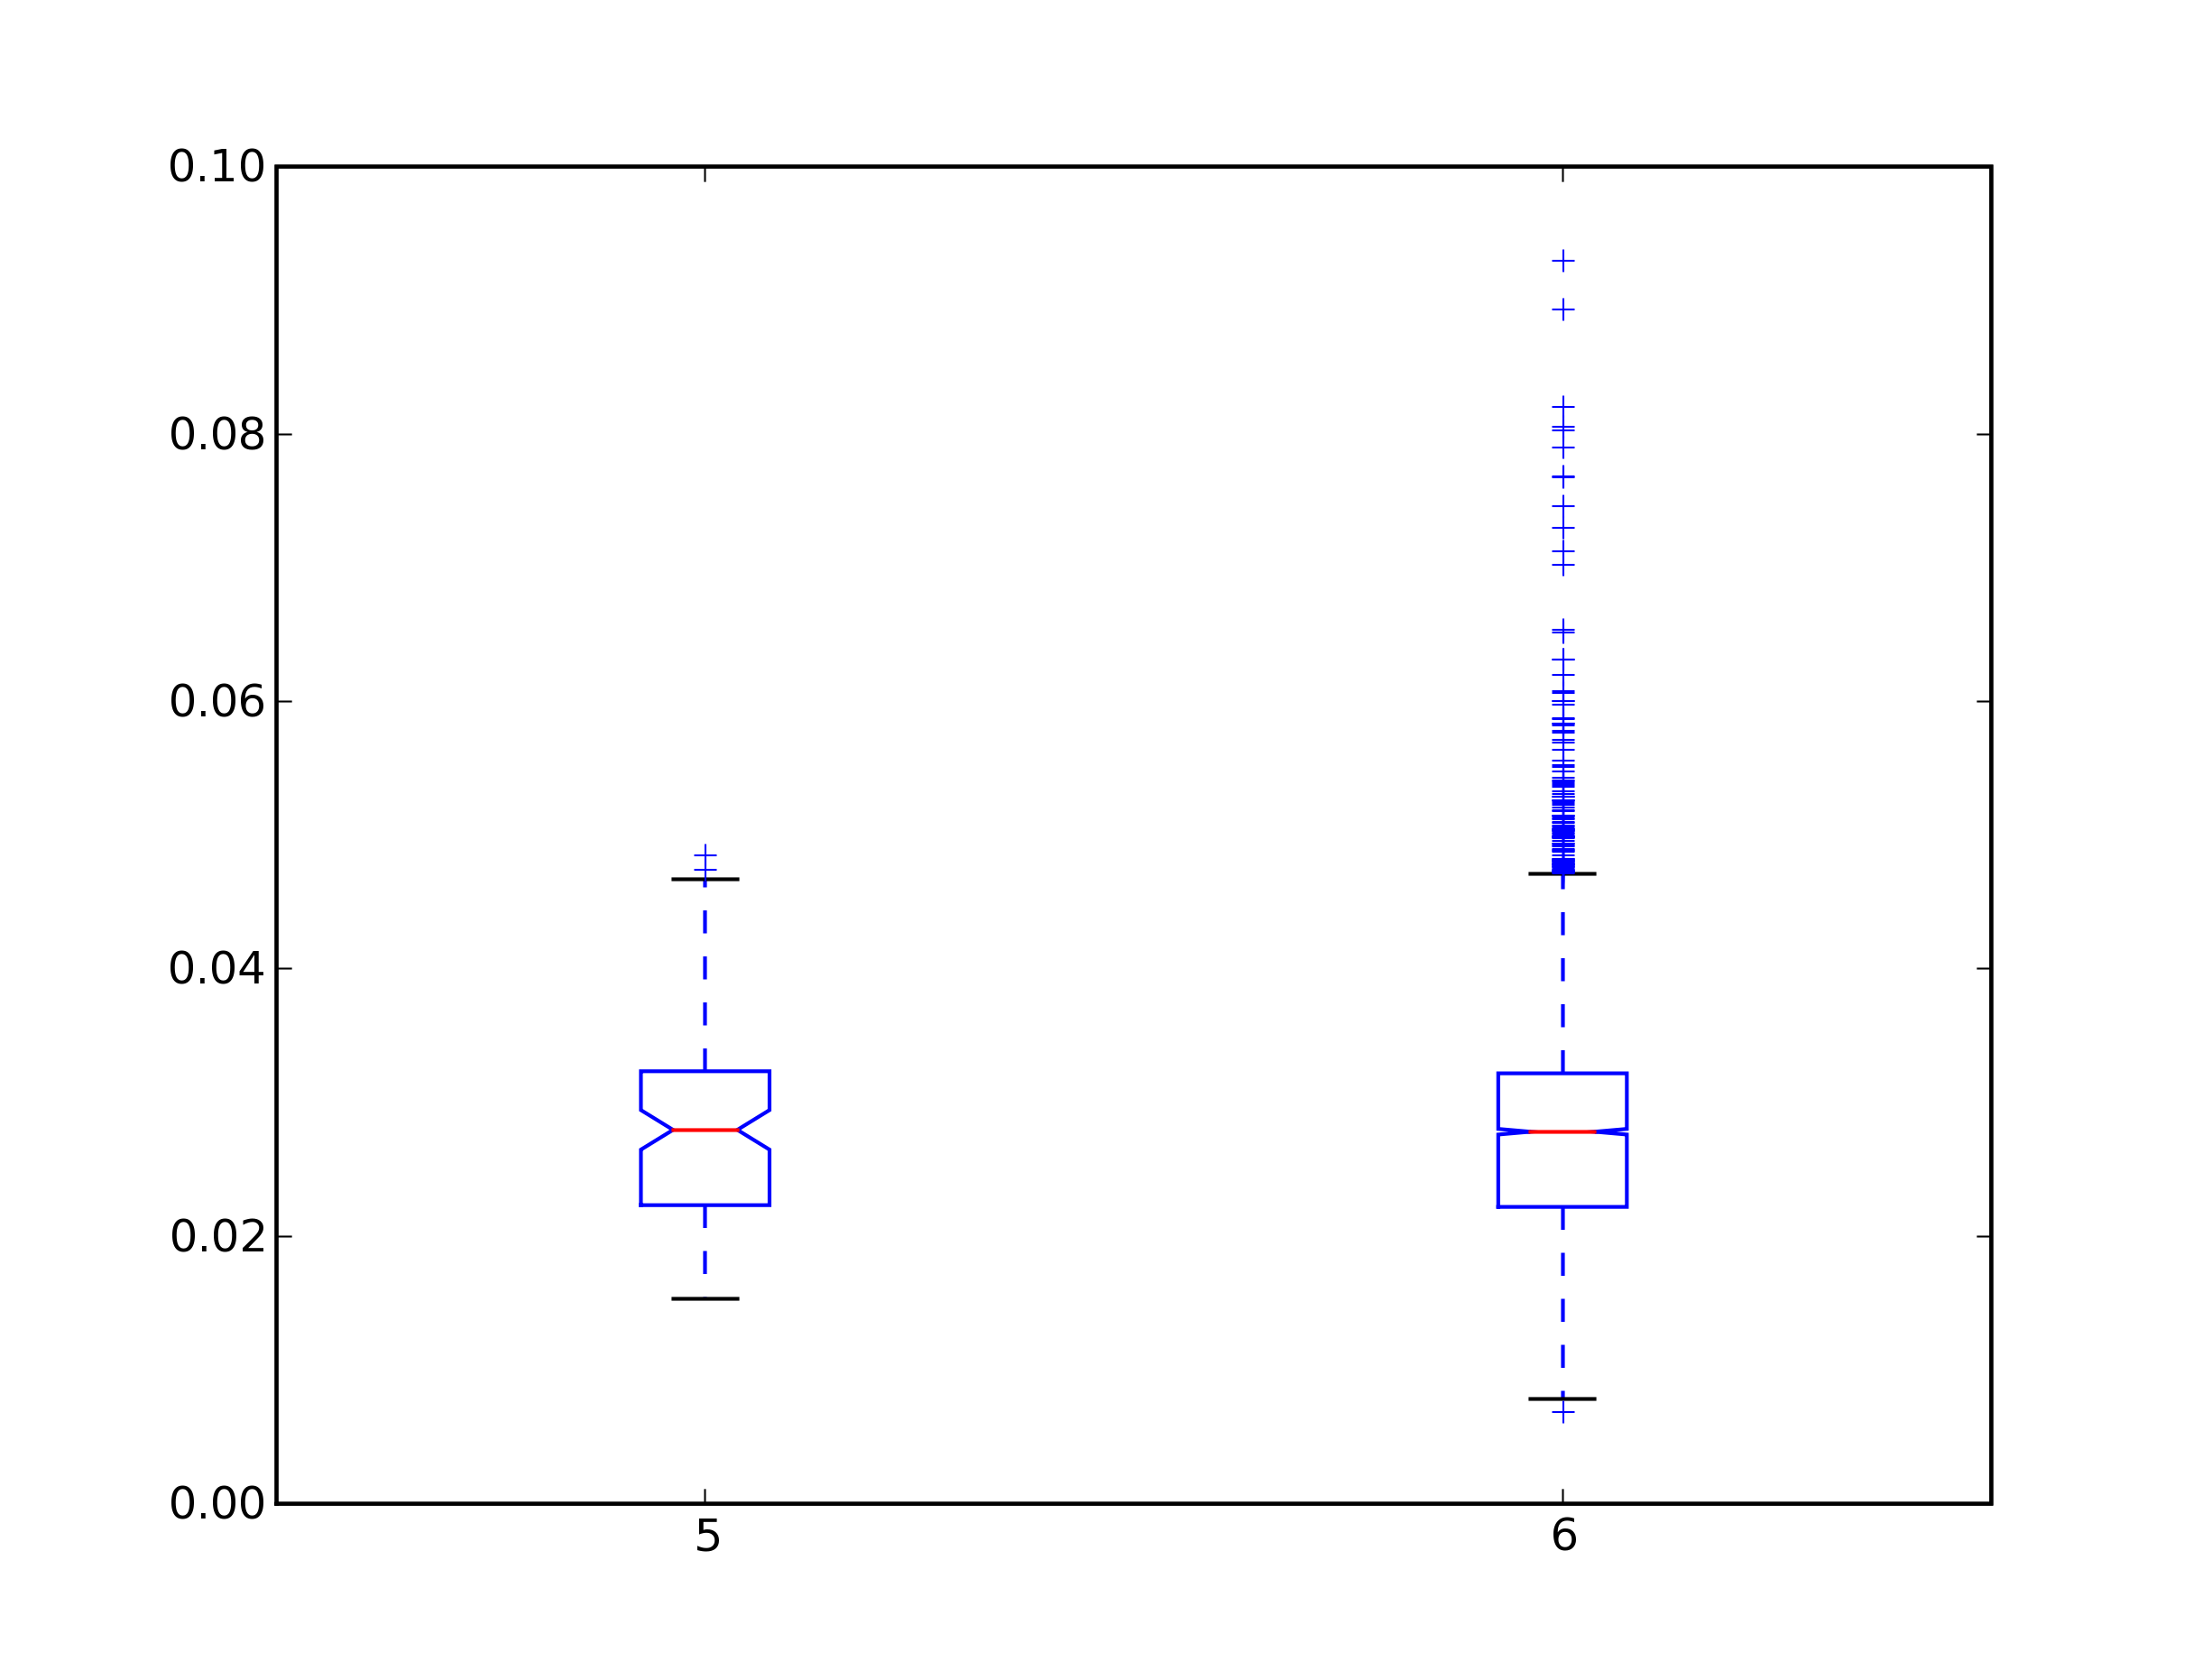
\includegraphics[width=\linewidth]{geodesic_iv_box.png}
\caption{This shows 4 box plots, each representing one group of neurons in a set
of SOMs trained with the same paremeters.}
\label{fGeodesicIV}
\end{figure}




To answer this question we need to setup a distance matrix (the distance of the
means) between each set of groups with in a given topology.  The table should
look like this...... 
\\
  2 3 4\\
2 0 + +\\
3 - 0 +\\
4 - - 0\\
\\
differance of means test\ldots
\ref{randomLabelTableRook}
\ref{randomLabelTableGraph}
\ref{randomLabelTableHex}
\ref{randomLabelTableGeodesic}

\begin{table}
\centering
\caption{Random Labeling Mean Tests for rook case,  delta (p-Value)}
\label{randomLabelTableRook}
\begin{tabular}{|c||c|c|c|}
\hline
&2&3&4\\
\hline
\hline
2& & 0.012681 (0.009000)& 0.024790 (0.001000)\\
\hline
3& 0.012681 (0.011000)& & 0.012109 (0.001000)\\
\hline
4& 0.024790 (0.001000)& 0.012109 (0.001000)& \\
\hline
\end{tabular} \end{table}


\begin{table}
\centering
\caption{Random Labeling Mean Tests for spherical case,  delta (p-Value)}
\label{randomLabelTableGraph}
\begin{tabular}{|c||c|c|c|}
\hline
&5&6&7\\
\hline
\hline
5& & 0.000362 (0.786000)& 0.001358 (0.480000)\\
\hline
6& 0.000362 (0.752000)& & 0.000996 (0.484000)\\
\hline
7& 0.001358 (0.503000)& 0.000996 (0.514000)& \\
\hline
\end{tabular} \end{table}

\begin{table}
\centering
\caption{Random Labeling Mean Tests for Hexgonal Lattice,  delta (p-Value)}
\label{randomLabelTableHex}
\begin{tabular}{|c||c|c|c|c|c|}
\hline
&2&3&4&5&6\\
\hline
\hline
2& & 0.004463 (0.525000)& 0.011735 (0.083000)& 0.017665 (0.011000)& 0.021821
(0.003000)\\
\hline
3& 0.004463 (0.548000)& & 0.007272 (0.006000)& 0.013202 (0.001000)& 0.017357
(0.001000)\\
\hline
4& 0.011735 (0.095000)& 0.007272 (0.002000)& & 0.005930 (0.014000)& 0.010086
(0.001000)\\
\hline
5& 0.017665 (0.012000)& 0.013202 (0.001000)& 0.005930 (0.019000)& & 0.004155
(0.060000)\\
\hline
6& 0.021821 (0.002000)& 0.017357 (0.001000)& 0.010086 (0.001000)& 0.004155
(0.056000)& \\
\hline
\end{tabular} \end{table}

\begin{table}
\caption{Random Labeling Mean Tests for Geodesic Lattice,  delta (p-Value)}
\label{randomLabelTableGeodesic}
\begin{tabular}{|c||c|c|}
\hline
&5&6\\
\hline
\hline
5& & 0.001476 (0.601000)\\
\hline
6& 0.001476 (0.584000)& \\
\hline
\end{tabular} \end{table}





